\chapter{Opis struktury Projektu}
\label{cha:opisStrukturyProjektu}


\section{Cała Struktura Projektu}
\begin{figure}[h!]
    \centering
    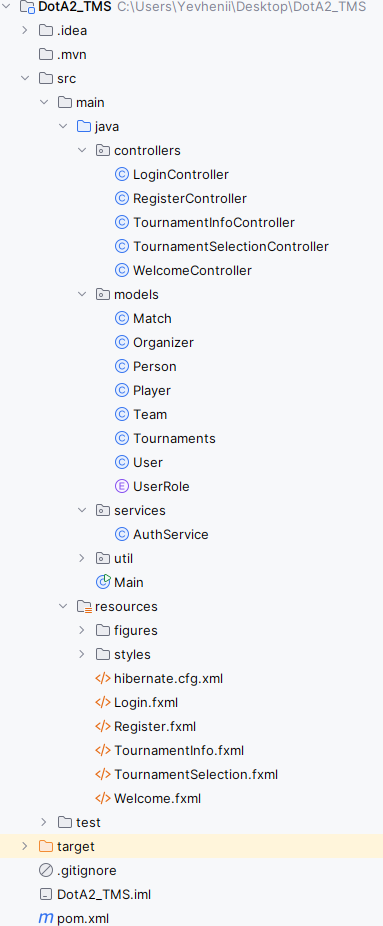
\includegraphics[width=0.5\textwidth]{figures/Structure.png}
    \caption{Struktura całego projektu \label{fig1}}
\end{figure}
\begin{figure}[h!]
    \centering
    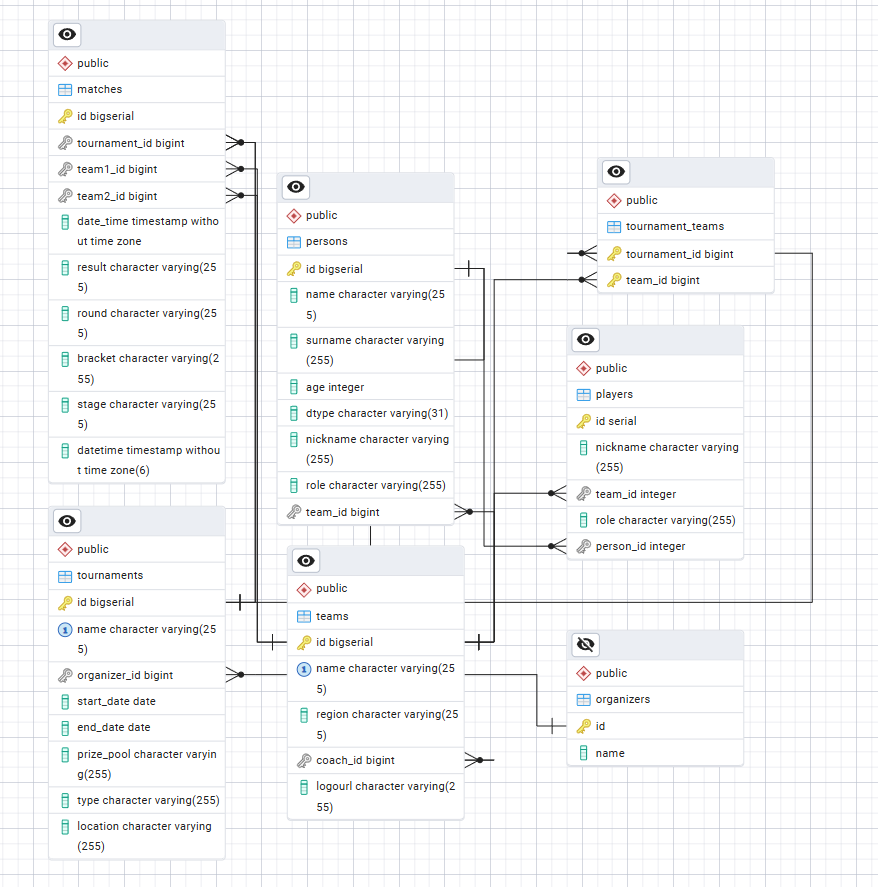
\includegraphics[width=0.8\textwidth]{figures/Database.png}
    \caption{Baza danych \label{fig2}}
\end{figure}

\subsection{Main}

Main po prostu uruchamia aplikacje i ustawia ikonę i title dla programu, zaczyna się ona od \texttt{Welcome.fxml}(interfejs zademonstruje w następującym rozdziale).

\lstinputlisting[caption= Main: jak zaczyna się program, label=JavaListing, style = javaStyle, firstline=8, lastline=24]{src/Main.java}


\subsection{Util and Service}
\lstinputlisting[caption= Klasa HibernateUtil: odpowiedzialna za konfigurację bazy danych, label=JavaListing, style = javaStyle, firstline=5]{src/HibernateUtil.java}

\lstinputlisting[caption= Klasa AuthService: autoryzacja z wyszukiwaniem w bazie konta i dehashowaniem hasła BCryptem, label=JavaListing, style = javaStyle, firstline=17, lastline=34]{src/AuthService.java}

\lstinputlisting[caption= Klasa AuthService: rejestracja ze sprawdzeniem czy istnieje już konto i hashowanie hasła nowego użytkownika, label=JavaListing, style = javaStyle, firstline=44, lastline=66]{src/AuthService.java}

\subsection{Controllers}
Pakiet \texttt{controllers} zawiera klasy odpowiedzialne za backend fxml plików. 

\begin{figure}[H]
    \centering
    \caption{Metody kontrolerów \label{fig4}}
    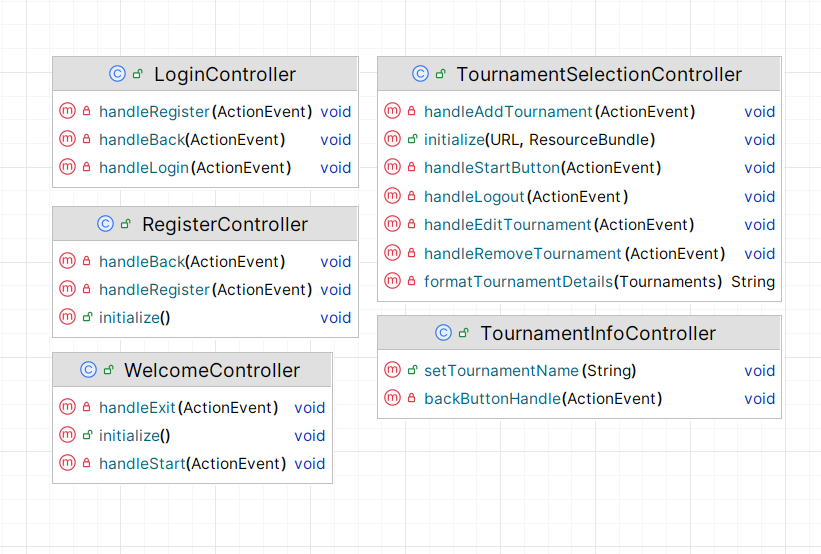
\includegraphics[width=0.8\textwidth]{figures/ControllersMethods.png}
\end{figure}

\lstinputlisting[caption= Klasa LoginController: handleBack i handleRegister - przekazania na nowe strony; handleLogin - logowanie użytkownika z wykorzystaniem wyżej opisanym AuthService dla autentyfikacji usera i przy poprawnych danych - przekazanie na nową stronę, label=JavaListing, style = javaStyle, firstline=32, lastline=92]{src/LoginController.java}

\lstinputlisting[caption= Klasa RegisterController: handleRegister - rejestracja nowego użytkownika z wykorzystaniem AuthService; umożliwia rejestrację jako Admin za pomocy sprawdzenia adminCodeField (admin code = 1111); obsługuje już istniejące lub puste dane, label=JavaListing, style = javaStyle, firstline=27, lastline=86]{src/RegisterController.java}

\lstinputlisting[caption= Klasa TournamentSelectionController: w tej klasie przy inicjalizację jest kontrola roli użytkownika i zrealizowane CRUD na turniejach(używamy HibernateUtil opisany wyżej); W przyszłości ulepszę tę klasę, label=JavaListing, style = javaStyle, firstline=68, lastline=418]{src/TournamentSelectionController.java}


\subsection{Models}

Pakiet \texttt{models} zawiera klasy, które są mapowane na tabele w bazie danych.

\begin{figure}[H]
    \centering
    \caption{Pola i dziedziczenie klas, każda klasa ma gettery i settery, a także metodę ToString  \label{fig3}}
    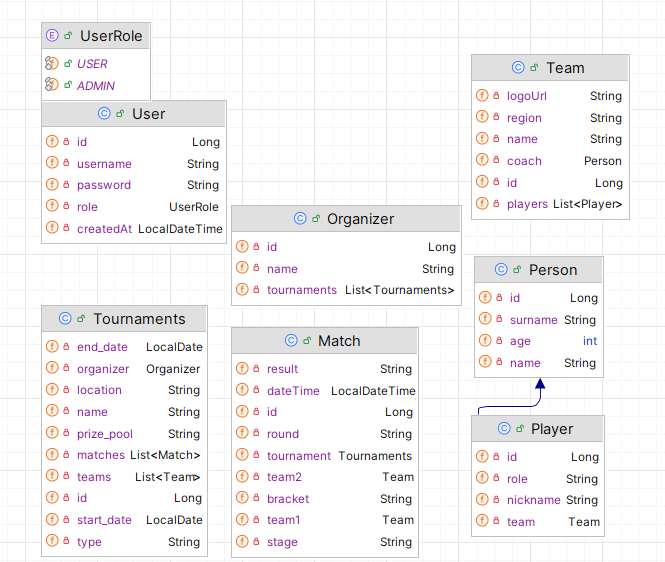
\includegraphics[width=0.8\textwidth]{figures/Classes.png}
\end{figure}

\lstinputlisting[caption= Przykład mapowania klas na klasie Tournaments, label=JavaListing, style = javaStyle, firstline=8, lastline=42]{src/Tournaments.java}

\subsection{Resources}
Pakiet \texttt{resources} zawiera pliki fxml, które są odpowiedzialne za wygląd aplikacji. Każdy plik jest rozpatrzony w następnym rozdziale.

Zawiera plik css, który daje ten ładny wygląd aplikacji, jest on wykorzystywany w każdym pliku fxml, aby zapewnić spójność stylu. Jest folder figures z obrazkami.

\section{Wykorzystane Technologie}
W projekcie wykorzystano następujące technologie:
\begin{itemize}
    \item \textbf{IntelliJ IDEA 2025.1.2} - IDE do tworzenia aplikacji w języku Java.
    \item \textbf{Maven 4.0.0} - budowanie projektu i zarządzanie zależnościami.
    \item \textbf{JavaFX 21.0.7} - projektowanie GUI.
    \item \textbf{JavaFX SceneBuilder} - projektowanie GUI.
    \item \textbf{PostgreSQL 17.5} - baza danych.
    \item \textbf{Hibernate 6.2.7} - warstwa ORM.
    \item \textbf{BCrypt} - bezpieczne hashowanie haseł.
\end{itemize}

\subsection{Wymagania sprzętowe}
Aby uruchomić aplikację, wymagany jest komputer z systemem operacyjnym Windows 10/11, Intellij Idea, Java 21, PostgreSQL i JavaFX 21.0.7.

Wszystko trzeba poprawnie skonfigurować, aby aplikacja działała poprawnie. W razie potrzeby wrzucę filmik z instrukcją repozytorium.

